\section{Self-Attention Defined}
\label{sec:self_attention}

\noindent
Traditional sequence processing faced several key challenges:
\begin{itemize}
    \item \textbf{Sequential bottleneck:} RNNs (Figure~\ref{fig:rnn_architecture}) process tokens one at a time, limiting parallelization
    \item \textbf{Information decay:} Long-range dependencies are hard to maintain through recursive state updates
    \item \textbf{Path length:} Information must flow through many intermediate steps to connect distant tokens
\end{itemize}

\begin{figure}[h]
\centering
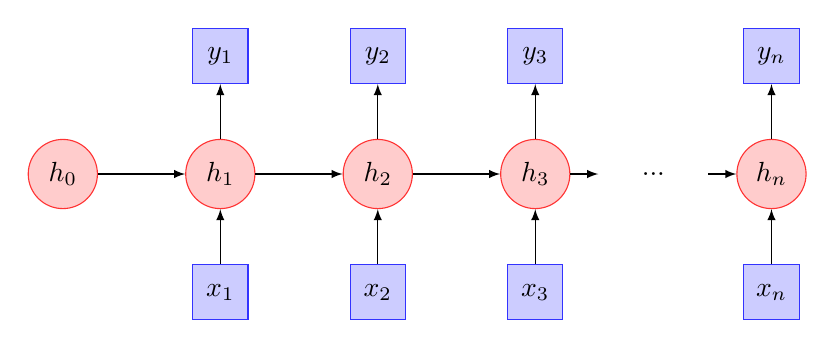
\begin{tikzpicture}[
    node/.style={circle, draw=red!80, fill=red!20, minimum size=25pt},
    box/.style={rectangle, draw=blue!80, fill=blue!20, minimum size=20pt},
    >=latex
]
    % RNN cells
    \node[node] (h0) at (0,0) {$h_0$};
    \node[node] (h1) at (2,0) {$h_1$};
    \node[node] (h2) at (4,0) {$h_2$};
    \node[node] (h3) at (6,0) {$h_3$};
    \node at (7.5,0) {...};
    \node[node] (hn) at (9,0) {$h_n$};
    
    % Input tokens
    \node[box] (x1) at (2,-1.5) {$x_1$};
    \node[box] (x2) at (4,-1.5) {$x_2$};
    \node[box] (x3) at (6,-1.5) {$x_3$};
    \node[box] (xn) at (9,-1.5) {$x_n$};
    
    % Output tokens
    \node[box] (y1) at (2,1.5) {$y_1$};
    \node[box] (y2) at (4,1.5) {$y_2$};
    \node[box] (y3) at (6,1.5) {$y_3$};
    \node[box] (yn) at (9,1.5) {$y_n$};
    
    % Horizontal connections
    \draw[->] (h0) -- (h1);
    \draw[->] (h1) -- (h2);
    \draw[->] (h2) -- (h3);
    \draw[->] (h3) -- (6.8,0);
    \draw[->] (8.2,0) -- (hn);
    
    % Vertical connections
    \draw[->] (x1) -- (h1);
    \draw[->] (x2) -- (h2);
    \draw[->] (x3) -- (h3);
    \draw[->] (xn) -- (hn);
    
    \draw[->] (h1) -- (y1);
    \draw[->] (h2) -- (y2);
    \draw[->] (h3) -- (y3);
    \draw[->] (hn) -- (yn);
\end{tikzpicture}
\caption{Recurrent Neural Network (RNN) architecture showing sequential processing. Information from token $x_1$ must pass through multiple hidden states ($h_1, h_2, ...$) to influence later predictions, creating a long path for learning long-range dependencies. Each hidden state $h_i$ depends on both the current input $x_i$ and the previous hidden state $h_{i-1}$, forcing sequential computation.}
\label{fig:rnn_architecture}
\end{figure}

\noindent
A core challenge in sequence modeling is capturing \emph{relationships between distant tokens} without relying on sequential processing. \textbf{Self-attention} solves this by allowing each token to attend to any other token in the sequence in \emph{parallel}, bypassing the bottlenecks of recurrence. In practice, self-attention is implemented using \textbf{queries}, \textbf{keys}, and \textbf{values}, which collectively determine how much each token “pays attention” to every other token.

\begin{figure}[h]
\centering
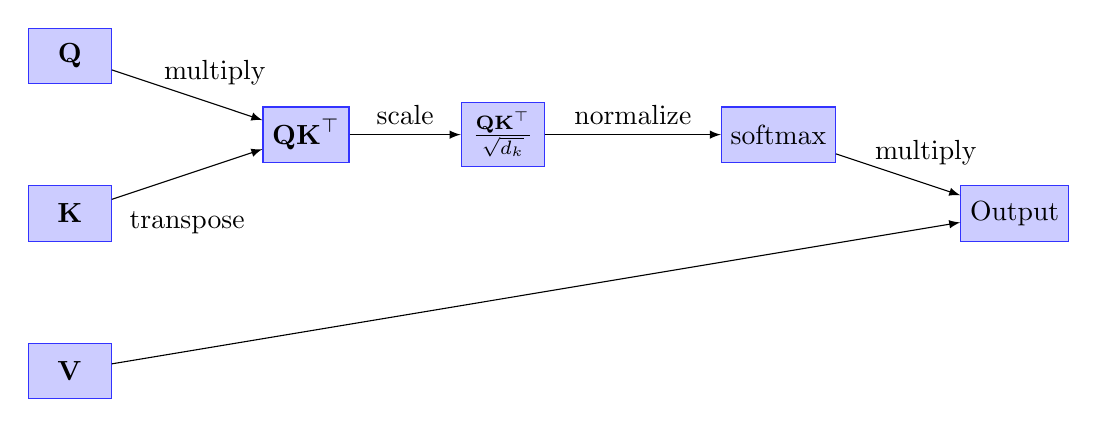
\begin{tikzpicture}[
    node/.style={rectangle, draw=blue!80, fill=blue!20, minimum size=20pt},
    matrix/.style={node, minimum width=30pt},
    vector/.style={node, minimum width=20pt},
    >=latex
]
    % Input matrices
    \node[matrix] (Q) at (0,2) {$\mathbf{Q}$};
    \node[matrix] (K) at (0,0) {$\mathbf{K}$};
    \node[matrix] (V) at (0,-2) {$\mathbf{V}$};
    
    % Matrix multiplication
    \node[matrix] (QK) at (3,1) {$\mathbf{QK}^\top$};
    
    % Scaling
    \node[matrix] (scaled) at (5.5,1) {$\frac{\mathbf{QK}^\top}{\sqrt{d_k}}$};
    
    % Softmax
    \node[matrix] (softmax) at (9,1) {softmax};
    
    % Final multiplication
    \node[matrix] (output) at (12,0) {Output};
    
    % Arrows and labels
    \draw[->] (Q) -- node[above, xshift=10pt] {multiply} (QK);
    \draw[->] (K) -- node[below, yshift=-10pt] {transpose} (QK);
    \draw[->] (QK) -- node[above] {scale} (scaled);
    \draw[->] (scaled) -- node[above] {normalize} (softmax);
    \draw[->] (softmax) -- node[above, xshift=10pt] {multiply} (output);
    \draw[->] (V) -- (output);
\end{tikzpicture}
\caption{Scaled Dot-Product Attention Mechanism. Queries ($\mathbf{Q}$), keys ($\mathbf{K}$), and values ($\mathbf{V}$) undergo matrix multiplications, scaling, and softmax normalization to produce weighted outputs. Each step is designed to ensure both expressive power and stable gradients.}
\label{fig:attention_mechanism}
\end{figure}

\subsection{Query, Key, and Value Formulation}
\noindent
To give each token direct access to the rest of the sequence, \textbf{three distinct representations} are learned:
\begin{itemize}
    \item \textbf{Query ($\mathbf{q}_i$)} – captures \emph{what} the current token \emph{wants to find} in the rest of the sequence
    \item \textbf{Key ($\mathbf{k}_i$)} – indicates \emph{what} the token \emph{can offer} or match on
    \item \textbf{Value ($\mathbf{v}_i$)} – stores the \emph{actual content} that might be retrieved if the match is relevant
\end{itemize}

\noindent
This query-key-value mechanism can be understood through an analogy to information retrieval:
\begin{itemize}
    \item Imagine searching in a library where:
    \begin{itemize}
        \item The \textbf{query} is like your search terms (e.g., "information about cats")
        \item The \textbf{keys} are like book titles or tags that can be matched against
        \item The \textbf{values} are the actual content of the books
    \end{itemize}
    \item In language understanding:
    \begin{itemize}
        \item A pronoun "she" might generate a \textbf{query} looking for female subjects
        \item Previous mentions of female names would have \textbf{keys} indicating they're potential antecedents
        \item The \textbf{values} would contain the full contextual information about those mentions
    \end{itemize}
\end{itemize}

\noindent
These vectors are produced by learned linear transformations of the input embeddings:
\[
    \mathbf{Q} = \mathbf{X}\mathbf{W}^Q, 
    \quad
    \mathbf{K} = \mathbf{X}\mathbf{W}^K, 
    \quad
    \mathbf{V} = \mathbf{X}\mathbf{W}^V,
\]
where $\mathbf{X}$ is the matrix of token embeddings, and $\mathbf{W}^Q, \mathbf{W}^K, \mathbf{W}^V$ are learnable parameter matrices. Each transformation serves a specific purpose:
\begin{itemize}
    \item $\mathbf{W}^Q$ projects tokens into a space that captures what information they need
    \item $\mathbf{W}^K$ creates representations that can be effectively matched against queries
    \item $\mathbf{W}^V$ transforms tokens into a form useful for downstream tasks
\end{itemize}

\noindent
The separation into queries, keys, and values enables the network to learn different aspects of token relationships:
\begin{itemize}
    \item Query-key compatibility determines \emph{which} tokens should interact
    \item Values determine \emph{what information} is exchanged in these interactions
    \item This separation allows more flexible information flow than direct token-to-token comparison
\end{itemize}

\subsection{Scaled Dot-Product Attention}
\noindent
Once queries, keys, and values are defined, the model computes \textbf{attention weights} to determine how much each query (token) should attend to each key:
\[
\text{Attention}(\mathbf{Q}, \mathbf{K}, \mathbf{V}) 
= \text{softmax}\Bigl(\frac{\mathbf{Q} \mathbf{K}^\top}{\sqrt{d_k}}\Bigr) \mathbf{V}.
\]
\begin{enumerate}
    \item \textbf{Dot-Product (Compatibility):} 
    $\mathbf{Q}\mathbf{K}^\top$ produces a raw score indicating how well a query matches each key.
    \item \textbf{Scaling:} 
    Dividing by $\sqrt{d_k}$ keeps the magnitude of these scores balanced as dimensionality grows—\emph{avoiding excessively peaked softmax outputs.}
    \item \textbf{Softmax (Normalization):} 
    Transforms raw scores into a probability distribution, ensuring that all attention weights sum to 1 for each query.
    \item \textbf{Value Aggregation:} 
    The probabilities are used to weight the \textbf{values} before summing. High-compatibility pairs contribute more information to the final output.
\end{enumerate}
This design \emph{explicitly} lets each token pull information from tokens most relevant to its query.

\subsection{Why the Scaling Factor Matters}
\noindent
Without the $\sqrt{d_k}$ divisor, dot products in high-dimensional spaces could become very large, causing \emph{vanishing} gradients after the softmax step. By dampening the dot-product values, we preserve stable gradients and prevent any single token from dominating attention simply due to high vector dimensionality. Formally, one may see this as a softmax \emph{temperature} term:
\[
\text{softmax}\Bigl(\frac{\mathbf{Q}\mathbf{K}^\top}{\sqrt{d_k}} \times \frac{1}{\tau}\Bigr)
\]
where $\tau = 1$ by default. Adjusting $\tau$ changes how “selective” the attention distribution is.

\subsection{Masked Self-Attention}
\noindent
For tasks like language modeling, we must maintain causality—i.e., not attend to future positions. This is done by adding a mask $\mathbf{M}$ before the softmax:
\[
\text{Attention}(\mathbf{Q}, \mathbf{K}, \mathbf{V}, \mathbf{M}) 
= \text{softmax}\Bigl(\frac{\mathbf{Q} \mathbf{K}^\top + \mathbf{M}}{\sqrt{d_k}}\Bigr) \mathbf{V},
\]
where entries in $\mathbf{M}$ are $-\infty$ for positions that should be inaccessible, effectively zeroing out those attention weights. This ensures that the model learns to generate tokens only based on \emph{previous} (or current) tokens.

\subsection{Computational Complexity and Implications}
\noindent
The self-attention operation requires $O(n^2 d_k)$ time for a sequence of length $n$, due to the pairwise computation of query-key scores. Here, $n$ represents the sequence length (number of tokens), which could be:
\begin{itemize}
    \item For language models: number of words/tokens in the input text (e.g., 512 tokens for BERT-base)
    \item For image transformers: number of patches (e.g., for a 224×224 image split into 16×16 patches, $n = 196$)
    \item For audio models: number of time-frequency segments
\end{itemize}

\noindent
Storing the attention scores requires $O(n^2)$ space because we need to maintain the full attention matrix where each token attends to every other token. For example:
\begin{itemize}
    \item A sequence of 1,000 tokens requires storing a 1,000 × 1,000 attention matrix
    \item For longer sequences like documents (e.g., 10,000 tokens), the quadratic scaling becomes prohibitive (100 million attention scores)
\end{itemize}

Despite the quadratic cost, self-attention allows \emph{parallel processing} of all tokens and provides a global receptive field. These advantages have led to various \emph{long-sequence} optimizations and variants, such as:
\begin{itemize}
    \item Sparse attention patterns
    \item Linear attention mechanisms
    \item Sliding window attention
    \item Hierarchical attention
\end{itemize}

However, the fundamental dot-product design remains central to modern Transformer-based architectures.

\begin{equation}\label{eq:attention_mechanism}
\text{Attention}(\mathbf{Q}, \mathbf{K}, \mathbf{V}) 
= \text{softmax}\Bigl(\frac{\mathbf{Q}\mathbf{K}^\top}{\sqrt{d_k}}\Bigr)\mathbf{V}
\end{equation}

\begin{equation}\label{eq:masked_attention}
\text{Attention}(\mathbf{Q}, \mathbf{K}, \mathbf{V}, \mathbf{M}) 
= \text{softmax}\Bigl(\frac{\mathbf{Q} \mathbf{K}^\top + \mathbf{M}}{\sqrt{d_k}}\Bigr) \mathbf{V}
\end{equation}

\begin{equation}\label{eq:mask_matrix}
M_{ij} = \begin{cases}
    0 & \text{if position } j \leq i \\
    -\infty & \text{otherwise}
\end{cases}
\end{equation}


\begin{pythoncode}[Scaled Dot-Product Self-Attention and Multi-Head Attention]
import torch
import torch.nn.functional as F

def self_attention(query, key, value, mask=None):
    """
    Compute scaled dot-product self-attention
    Args:
        query: torch.Tensor (batch_size, num_queries, d_k)
        key: torch.Tensor (batch_size, num_keys, d_k)
        value: torch.Tensor (batch_size, num_values, d_v)
        mask: Optional[torch.Tensor] (batch_size, num_queries, num_keys)
    Returns:
        attention_output: torch.Tensor (batch_size, num_queries, d_v)
        attention_weights: torch.Tensor (batch_size, num_queries, num_keys)
    """
    # Compute scaled dot-product attention scores
    d_k = query.size(-1)
    scores = torch.matmul(query, key.transpose(-2, -1)) / math.sqrt(d_k)
    
    # Apply mask if provided (e.g., for causal attention)
    if mask is not None:
        scores = scores.masked_fill(mask == 0, float('-inf'))
    
    # Compute attention weights with softmax
    attention_weights = F.softmax(scores, dim=-1)
    
    # Compute weighted sum of values
    attention_output = torch.matmul(attention_weights, value)
    
    return attention_output, attention_weights

class MultiHeadAttention(nn.Module):
    def __init__(self, d_model, num_heads):
        super().__init__()
        self.d_model = d_model
        self.num_heads = num_heads
        self.d_k = d_model // num_heads
        
        # Linear projections for Q, K, V
        self.W_q = nn.Linear(d_model, d_model)
        self.W_k = nn.Linear(d_model, d_model)
        self.W_v = nn.Linear(d_model, d_model)
        self.W_o = nn.Linear(d_model, d_model)
    
    def forward(self, x, mask=None):
        batch_size = x.size(0)
        
        # Linear projections and reshape for multiple heads
        q = self.W_q(x).view(batch_size, -1, self.num_heads, self.d_k).transpose(1, 2)
        k = self.W_k(x).view(batch_size, -1, self.num_heads, self.d_k).transpose(1, 2)
        v = self.W_v(x).view(batch_size, -1, self.num_heads, self.d_k).transpose(1, 2)
        
        # Compute attention for each head
        output, weights = self_attention(q, k, v, mask)
        
        # Concatenate and project back to d_model dimensions
        output = output.transpose(1, 2).contiguous().view(batch_size, -1, self.d_model)
        return self.W_o(output)
\end{pythoncode}
